\documentclass{article}
\usepackage{amsmath}
\usepackage{array}
\usepackage{color}
\usepackage{graphicx}
\usepackage{float} %utiliser H pour forcer � mettre l'image o� on veut
\usepackage{lscape} %utilisation du mode paysage
\usepackage{mathbbol} % permet d'avoir le vrai symbol pour les reels grace a mathbb
\usepackage{enumerate}
\usepackage{marvosym}	
\usepackage{moreverb} % permet d'utiliser verbatimtab : conservation la tabulation 


\setlength {\textwidth}{16cm}
\setlength {\textheight}{21cm} 
\setlength {\oddsidemargin}{0cm}
\setlength{\headsep}{5pt} 

\newcommand\bn{\boldsymbol{\nabla}}
\newcommand\bo{\boldsymbol{\Omega}}
\newcommand\br{\mathbf{r}}
\newcommand\la{\left\langle}
\newcommand\ra{\right\rangle}
\newcommand\bs{\boldsymbol}

\renewcommand{\(}{\left(}
\renewcommand{\)}{\right)}
\renewcommand{\[}{\left[}
\renewcommand{\]}{\right]}

\newtheorem{theorem}{Theorem}[section]

\begin{document}
\title{\textsc{\huge{Project : optimization for radiotherapy}}}
\author{Bruno Turcksin} 
\date{}
\maketitle

\section{Introduction}

The modern radiotherapy uses the Intensity Modulated Radiation Therapy (IMRT) as one of the methods to treat cancer. IMRT allows to have several beams with different intensity profiles. The goal is to give a sufficient dose to the tumor while sparing healthy organs. To optimize the intensity profile, it is very common to divide the beams in small beamlets. Each beamlet has a constant intensity. In a real application, the number of beamlets is around a thousand. 

This problem is very complex and a lot of objective functions and constraints \cite{math}, \cite{complexity}, \cite{minima},\cite{dose-volume} have been proposed. Moreover, there is a lot of methods \cite{dose-volume} used to solve these optimization problems. We will use only 2 different optimizations. The first one because the problem is easy to solve and the second because it is a more realistic problem. 

\section{First objective function}
\subsection{Equations}
The first objective function comes from \cite{math} and is given by :
\begin{equation}
\min \(\theta_{\mathcal{T}} \sum_{(i,j)\in \mathcal{T}} \(D_{ij}-\delta_{ij}\)^2 + \theta_{\mathcal{R}} \sum_{(i,j)\in \mathcal{R}} \(D_{ij}-\delta_{ij}\)^2 + \theta_{\mathcal{N}} \sum_{(i,j)\in \mathcal{N}} \(D_{ij}-\delta_{ij}\)^2\)
\end{equation}
$\theta_{\mathcal{T}}$ is the target weight, $\theta_{\mathcal{R}}$ is the region at risk weight, $\theta_{\mathcal{N}}$ is the normal tissue weight and $\delta_{ij}$ is the prescribed dose for the pixel $ij$.\\

$D$ is a matrix which represents the total dose delivered to a transverse cross section of the patient, and it is equal to the sum over all beamlets $p$ of the beam weight multiplied by its corresponding dose matrix $D^p$ :
\begin{equation}
D_{ij} =  \sum_{p=1}^n w_p D_{i,j}^p
\end{equation}
where $n$ is the number of beamlets, $i$ and $j$ are the voxel coordinates.

The objective function is quadratic but there are some constraints since it is not possible to have the intensity of the beams negative (we can also impose the dose to be positive or zero everywhere). Here we should notice that unlike a real application, we do not solve the coupled photon-electron transport but only the simpler photon transport. The equation is :
\begin{equation}
\bo\cdot \Psi(\br,\bo,E) + \Sigma_t(\br,E) \Psi(\br,\bo,E) = \int_{4\pi} \Sigma_s(\br,\bo\cdot\bo',E) \Psi(\br,\bo',E)d\bo'+ S(\br,\bo,E)
\end{equation}
where $S$ is a volumetric source. $\Psi(\br,\bo,E)$ is related to $\Phi(\br,E)$ by :
\begin{equation}
\Phi(\br,E) = \int_{4\pi} \Psi(\br,\bo,E) d\bo
\end{equation}
The intensity of the beams, $J_i$, will be used through the boundary conditions :
\begin{equation}
J_i = \int_0^{\infty}\!\!\!\int_{\mathcal{D}_i} \Phi(\br,E)\ d\br\ dE
\end{equation}
where $\mathcal{D}_i$ is a part of the boundary ($\mathcal{D}_i\cap \mathcal{D}_j = \delta_{ij}\mathcal{D}_i$).
To solve this problem, we use a 2D transport code. The optimization part is written in Python. Since the objective function is quadratic, a Newton method seems perfect. However, because of the constraints, we cannot expect, in the general case, to converge in only one iteration. To solve this problem, we chose to use a BFGS method which is already implemented in the optimization library of Python\cite{python}. This function uses BFGS to solve a constrained problem and uses also line search. 

\subsection{Results} \label{testcarre}
We show here a few results that we have. We start with a one energy group problem. The domain is a square and we allow to have 20 beams. Each beam is orthogonal to the boundary. We want the dose to be zero except in the middle of the square, where we want it to be one. We show here 3 results :
\begin{enumerate}
\item $\theta = 1$ for all the cells
\item $\theta = 10$ for all the cells
\item $\theta = 10$ for all the cells and we force the symmetry of the problems. We know that we should have only 3 different intensities for the 20 beams.
\end{enumerate}

\subsubsection{$\theta = 1$}
We have the following result :
\begin{figure}[H]
\centering
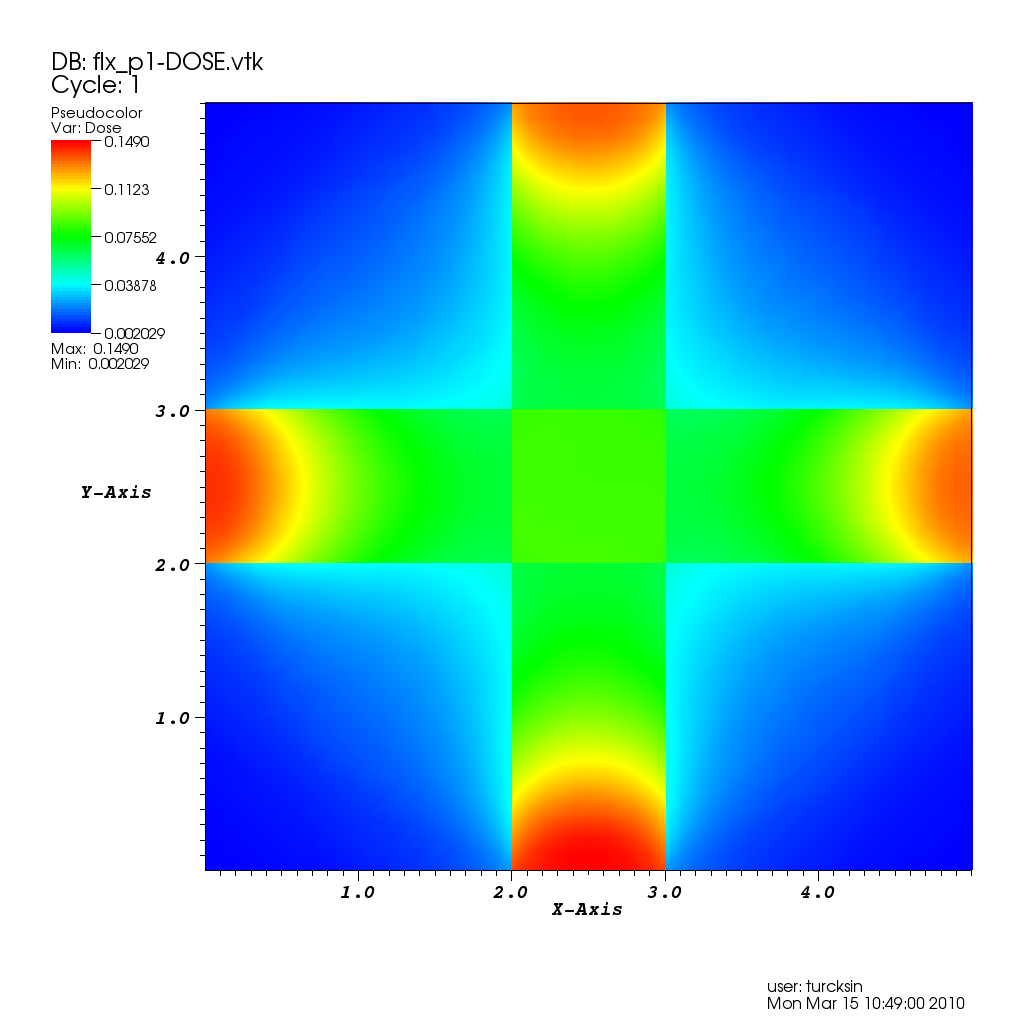
\includegraphics[width=0.5\linewidth]{theta_1}
\end{figure}
As expected, we have only 4 beams (the others are turned off since they cannot reach the target). The values of the for beams is given by :
\begin{table}[H]
\centering
\begin{tabular}{|c|c|c|c|c|}
\hline
Beam & 1 & 2 & 3 & 4\\
\hline
Intensity & 0.42429688 &  0.40194908 & 0.44576713 & 0.40617629\\
\hline
\end{tabular}
\end{table}
The value of the objective function is 0.918498315027. The time needed to solve this problem is quite long. It takes only 2.5 seconds to solve the transport problem but the whole optimization took more than 30 minutes. It is also interesting to notice that the intensities of the beams are not the same every where. There is 10\% of difference between them.

\subsubsection{$\theta = 10$}
The shape of the solution is exactly the same but we have some few differences. The values of the four beams is given by :
\begin{table}[H]
\centering
\begin{tabular}{|c|c|c|c|c|}
\hline
Beam & 1 & 2 & 3 & 4\\
\hline
Intensity &0.41434637 &   0.42877742 & 0.41759019 & 0.40841102\\
\hline
\end{tabular}
\end{table}
The value of the objective function is 9.18397683418. Solving the optimization problem takes less time than before (around 23 minutes). We can see that the objective function is slightly slower than the previous one. The intensities are also more closer to each other than the previous one.

\subsubsection{$\theta = 10$ and we force symmetry}
The shape of the solution is exactly the same but we have some few differences. The values of the for beams is given by :
\begin{table}[H]
\centering
\begin{tabular}{|c|c|c|c|c|}
\hline
Beam & 1 & 2 & 3 & 4\\
\hline
Intensity &0.38847929 &   0.38847929 & 0.38847929 & 0.38847929\\
\hline
\end{tabular}
\end{table}
The value of the objective function is 9.18456807572. We see a very interesting things here. The objective value is slightly higher than in the previous case and the intensity is slower.

\section{Second objective function}

\subsection{Equations}
The second objective function is closer of what is used in real application. The objective function is :
\begin{equation}
\min  \sum_{(i,j)\in \mathcal{T}} \(D_{ij}-\delta_{ij}\)^2 
\label{objective}
\end{equation}
So now we just want to minimize the difference between the planned dose and the dose in the tumor. The main difference with the previous problem comes from the constraints. Now we use dose-volume constraints \cite{complexity}, \cite{minima} and \cite{dose-volume}. The idea is that we do not want have more than a given percentage of the volume of an organ to receive more than a given dose. Mathematically, we have for each constraint :
\begin{equation} 
\sum_{ij \in \mathcal{D}} \nu\(D_{ij}-\delta_{ij}\)\frac{V_{ij}}{V} \leq \gamma
\label{constraint}
\end{equation}
where $V_{ij}$ is the volume of voxel $ij$, $V$ is the total volume of the organ, $\nu(x)$ is the Heaviside function and $\gamma$ is the tolerance percentage volume. We also impose the dose to be positive or zero :
\begin{equation}
D_{ij} \geq 0
\label{constraint2}
\end{equation}

\subsection{Local minima}
It is well known that even if the objective function is convex, the problem has several local minima \cite{minima}. The reason is that the domain is not convex. The number of local minima can increase factorially with the number of beamlets. Since we can have more than a thousand of beamlets, we see that the number of local minima can be huge. We can also write the problem as a mixed-integer linear problem. This kind of problem does not have the problem of having a lot of local minima but the calculation time can be prohibitive \cite{minima}.

Now we show 3 examples where we use the dose-volume constraint. 
\subsubsection{Test 1} \label{test1}
In the first case, we use the same problem than the previous section. We have the tumor in the middle of a square and we want a dose of 1. We do not want that more than 10\% of the healthy organ receives a dose larger than 0.1. We have two beams, one coming from the left and one from the bottom. We show here the value of the objective function :
\begin{figure}[H]
\centering
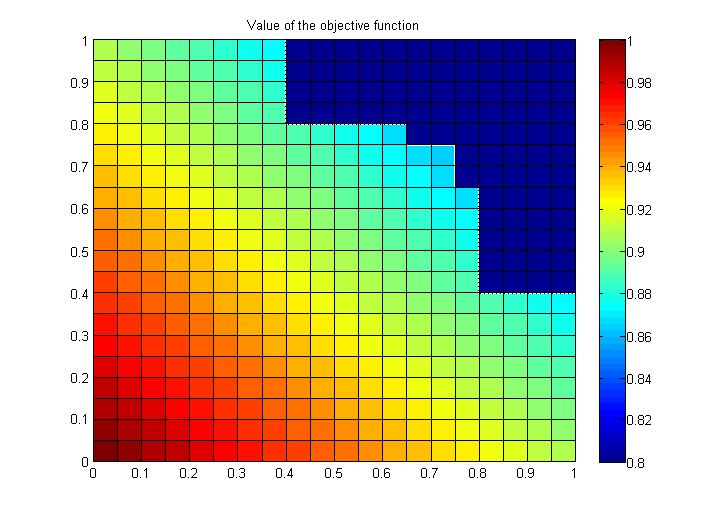
\includegraphics[width=0.5\linewidth]{dv_of_1}
\end{figure}
The area in dark blue is the forbidden area. We see that there are several minima. It seems that there are 5 minima but 2 of them are probably due to the mesh. If we refine the mesh, they would disappear. So we have 3 minima with 2 of them which have the same value : $f=0.8686$. The last minimum has a value of : $f=0.8640$. We must notice that we probably do not have the actual global minimum. For the 2 minima of $f=0.8686$, we could probably have some improvement if we take some higher intensities for the beams. Effectively, we can have a much larger beam-intensity when the 2 beams are not symmetric. This is because of the way the constraints are built : it does not matter if the dose is 1\% higher than the given dose or 100\% higher. That is why it is probably better to have 2 different intensities for the 2 beams.
%The area in dark blue is the forbidden area. We see that there is 3 minima. Two of them have the same value and are the global minima : $f=0.8702$. We also have another minimum $f=0.9018$. This minimum appears when the two beams have the same intensity. It is not obvious at first sight that this minimum is only a local minimum and not the global minimum. However, if we look back at the constraint, we see that the constraint is active as soon as a given volume receive more than a given dose. It does not matter if the dose is 1\% higher than the given dose or 100\% higher. In this case, we see that the best solution is to have a beam with a big intensity and one with much less. If the two beams have the same intensity, we could decrease the maximum dose receive by a cell but more cells would receive an important dose.
\subsubsection{Test 2} \label{test2}
The second case is very similar to the previous one but now, the tumor is bigger. We assume that the voxel in the middle of the square and the voxel just below it, are the tumor. The objective function looks like that :
\begin{figure}[H]
\centering
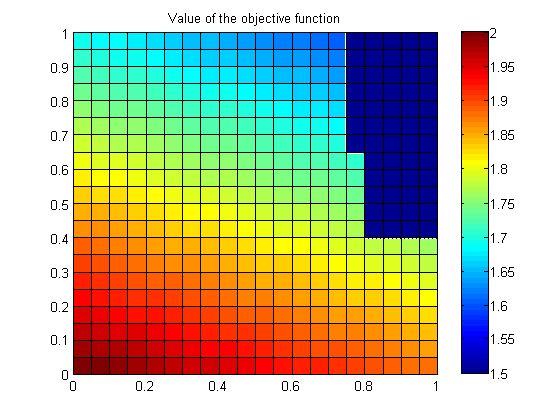
\includegraphics[width=0.5\linewidth]{dv_of_2}
\end{figure}
We see that there is only 3 minima. One when the beam from below has the biggest intensity ($f=1.597$), one when the beam from the left has the biggest intensity ($f=1.7553$) and the last one when the 2 beams are strong ($f=1.7074$). We see that we have more than 10\% of difference in the objective value if we choose the first or the second intensity. This difference could be larger if we had allowed to have a larger intensity for the beams.
\subsubsection{Test 3}\label{test3}
Finally, we show what happened when we decrease the maximum dose allowed. The problem is the same than the previous one but the maximum dose for the healthy cells is 0.05. The objective function looks like :
\begin{figure}[H]
\centering
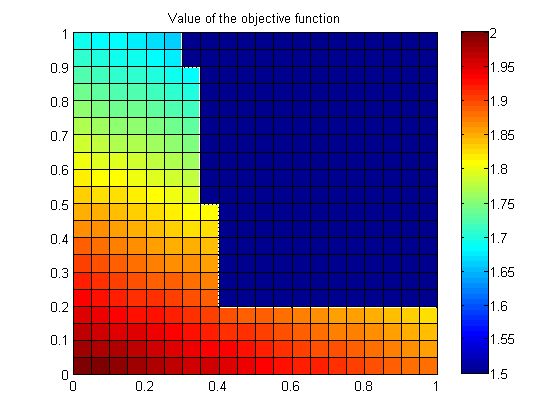
\includegraphics[width=0.5\linewidth]{dv_of_3}
\end{figure}
There are 4 minima :
\begin{align}
& f = 1.8199\\
& f = 1.8054\\
& f = 1.6856\\
& f = 1.6459
\end{align}
We see that even with a simple case we have several minima. The difference in the objective function for 2 ``extreme'' minima is around 10\% in the last case. We can expect to have many more minima when we increase the number of beams to have a bigger difference between several local minima. 

\subsection{Algorithm}
It seems obvious than we need a method like the simulated-annealing. This method can deal easily with a lot of minima. The only problem is that this method converges very slowly like all the stochastic methods. Instead, we will try to use a deterministic method to find a good approximation of the global minimum. We will use the Newton method with the following steps (we use a similar method that \cite{dose-volume}) :
\begin{enumerate}
\item we optimize the dose without any constraint.
\item we sort the voxel in the healthy organs by their received dose from a low dose to a high dose.
\item we apply the constraint $D_{ij} < \delta_{ij}$ on the $\(1-\gamma\)N$ voxels with the lowest dose ($N$ is the number of voxels for the organ) for each organ. 
\item We solve the optimization problem (active set).
\item we go back at the step 2 until the solution cannot be improved anymore.
\end{enumerate}
So we see that at the third step, we need to use the active set method. Since for the first step, we solve the unconstrained problem, which will give us the lower bound for the constrained problem, and then we try to stay close by imposing the constraints on the voxels with the lowest dose, we can hope that we will not be too far from the global minimum. We should be able to solve quickly the active set method since we have a good approximation of the solution and we know what should be the initial working set.

Unlike for the first objective function, we will have to write most of the algorithm ourselves. That will allow us to avoid some calculations. We know that we will need to compute the gradient of (\ref{objective}), (\ref{constraint}) and (\ref{constraint2}) (we assume that there is only group and that we apply the algorithm described before) :
\begin{align}
& \bn f = \sum_{(i,j)\in \mathcal{T}} 2 \(D_{i,j}-\delta_{i,j}\) \Sigma_{a,ij}\bn\Phi_{ij}\\
& \bn h = -\Sigma_{a,ij}\bn\Phi_{ij}\ \ \ \ \forall (i,j) \in \mathcal{P} \\
& \bn h = \Sigma_{a,ij}\bn\Phi_{ij} \ \ \ \ \forall (i,j)
\end{align}
where $\bn \Phi_{ij}$ is the gradient of the flux with respect of the intensity of the beams and $\mathcal{P}$ is the region which has to satisfy the constraint $D_{ij}<\delta_{ij}$.

We see that we need to compute $\bn \Phi_{ij}$ but $\Phi_{ij}$ is a linear function of the intensity of the beams. Thus, the gradient is constant and we can compute it once for all at the beginning of the calculation. Since $\bn \Phi_{ij}$ is constant, we have :
\begin{align}
& \bn^2 f = \sum_{(i,j)\in \mathcal{T}} 2 \Sigma_{a,ij}^2 \bn\Phi_{ij}\cdot\bn\Phi_{ij}^T\\
& \bn^2 h = 0
\end{align}
Thus, we can compute the global Hessian once for all, as soon as we have $\bn \Phi_{ij}$. This Hessian includes all the constraints so we will need to take a submatrix of it when we solve the problem.

\subsection{Previous results}
We show here the first results that we already showed in the previous report i.e. the solution for the problem without constraints. We do not have to worry about some beams with negative intensity since we do not want to spare any organs. Thus, we have a quadratic objective function and we do not have any constraints. We can expect to solve this problem with only one Newton iteration. Unfortunately, the Hessian is not positive definite but semi-positive definite. Thus, we cannot invert the Hessian. So we modified the Hessian\footnote{Like in the Levenberg-Marquardt method} by adding the identity matrix multiplied by $10^{-8}$. In this way, we have avoid to have a singular matrix. However, the matrix can be very ill-conditioned since the lowest eigenvalue is now $10^{-8}$. To avoid that we modify the Hessian by multiplying each element on the diagonal of the Hessian by $1+10^{-8}$. Now, we avoid to have an ill-conditioned matrix. We show here the results given by the 2 methods :

\subsubsection{Levenberg-Marquardt method}
We want to have a dose of 1 in the square in the middle of the domain. The dose is : 
\begin{figure}[H]
\centering
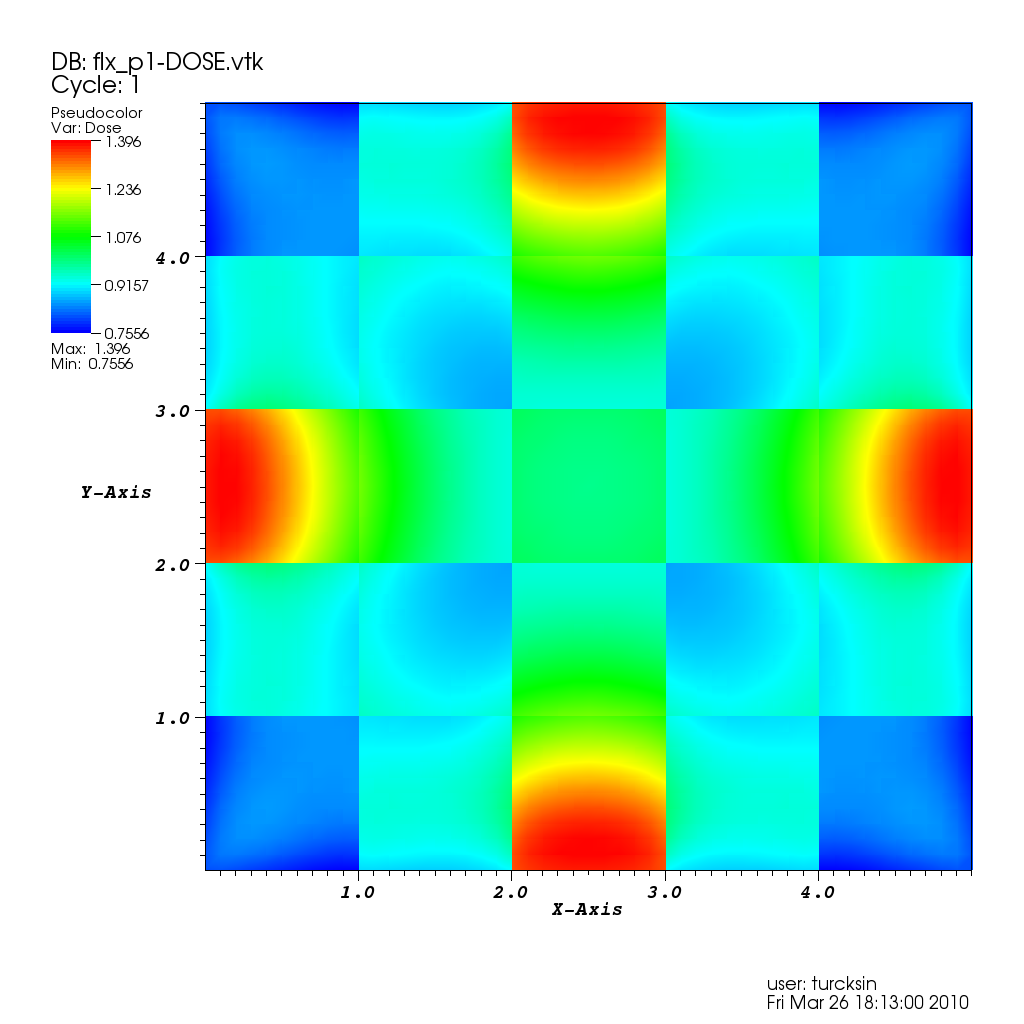
\includegraphics[width=0.5\linewidth]{L_M}
\end{figure}
We see that we have what we expected, the 4 beams which can reach the source without any scattering have the biggest intensity. The beams on the corners, which need a lot of scattering to get to the target, have the smallest intensity.

\subsubsection{Scaling method} 
Like in the previous case, we want a dose of 1 in the middle of the domain. The dose is :
\begin{figure}[H]
\centering
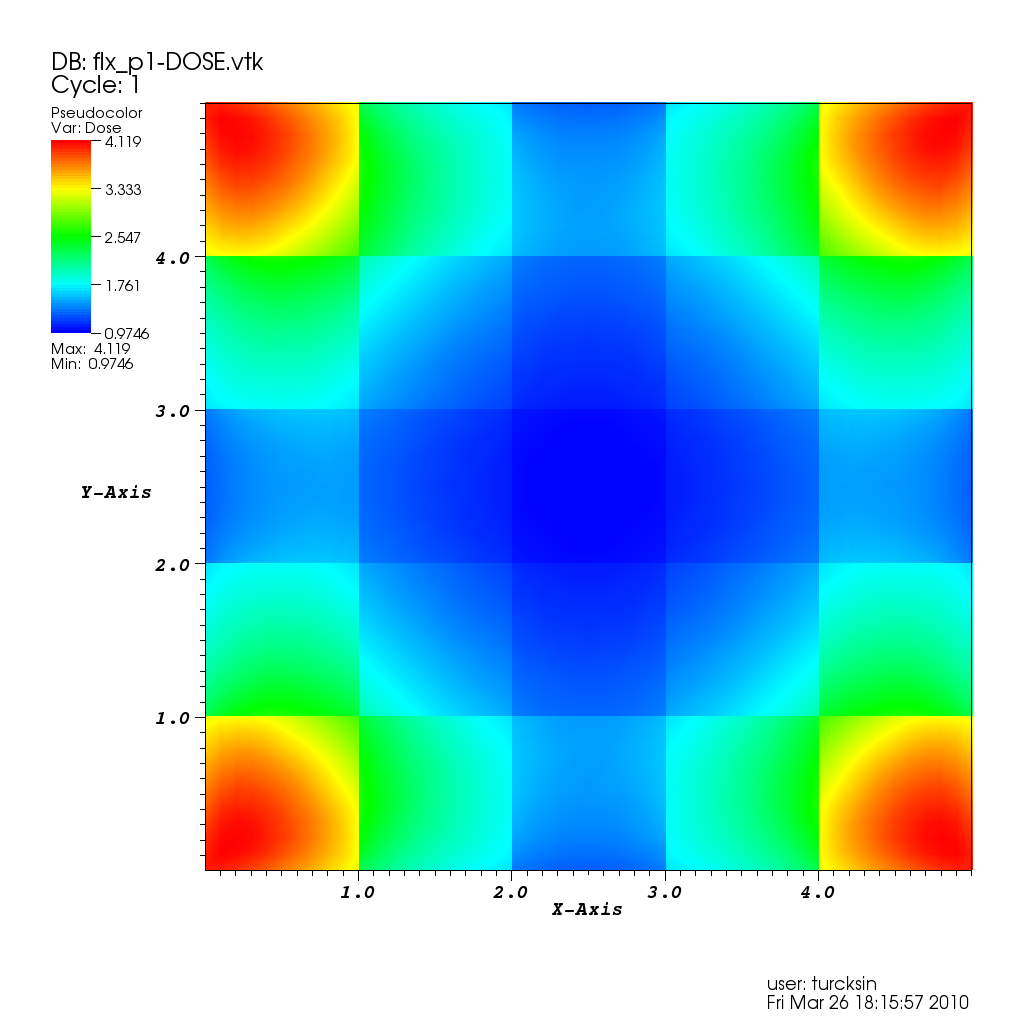
\includegraphics[width=0.5\linewidth]{N_L_M}
\end{figure}
We have basically the opposite of the previous case, the beams on the corners have the biggest intensities and the ones in the middle have the smallest intensities. Here the target is the area which has the lowest dose. We should notice that even if the 2 Hessian are almost the same, the answer is very different. In both case, we have the right dose but the intensity of the beams is very different.

\subsection{2 beams}
Now we go back the previous tests with the 2 beams.
\subsubsection{Test 1}
If we don't have any constraints, the intensity of the beams is 9.9283886 for the 2 beams and the value of the objective function is $9.67764\times 10^{-13}$. If we use the ``Levenberg-Marquardt'' method, we find that the intensity of the beams is 0.73463166 and that the value of the objective function is 0.857489 in 17s. If we use the scaling method, we find the same result in the same time. We see that we did not escape the local minimum (see \ref{test1}). The optimal solution of the constrained problem is  too far from the optimal solution of the unconstrained problem. We allow only 2 cells to receive a high dose and thus, these 2 cells are the 2 cells on the border which receives the beams. The method does not ``turn off'' one beam so it can increase the intensity of the other.
\subsubsection{Test 2}
If we don't have any constraints, the intensity of the beam coming from the left is 13.3355 and the intensity of the beam coming from below is 6.5213. The value of the objective function is $1.92578\times 10^{-16}$. If we use the ``Levenberg-Marquardt'' method, we find that the intensity of the left beam is 0.40434 and the intensity of the beam coming from below is 3.13236. The value of the objective function is 1.05058 in 18s. If we use the scaling method, we find the same result in the same time. This time, we see that we did not get stuck in a local minimum and that the beam from below has a bigger intensity than the left beam like it should. The result is quite good and we do what we expected (see \ref{test2}).
\subsubsection{Test 3}
Of course, we have the same results for the unconstrained problem. If we use the ``Levenberg-Marquardt'' method, we find that the intensity of the left beam is 0.20217 and the intensity of the beam coming from below is 1.56618. The value of the objective function is 1.4848 in 18s. If we use the scaling method, we find the same result in the same time. Like previously, we find the result that we expected (see \ref{test3}).

\subsection{20 beams}
Now we will show an example similar to the one in section \ref{testcarre}.  The difference is that we do not choose the value of $\theta$ but the maximal dose and the ratio of the volume which can receive a higher dose. Here we want to have a dose of 1 in the middle cell and we do not want to have more than 50\% of the cells to receive a dose higher than 0.1.
\subsubsection{Levenberg-Marquardt method}
Here we show the result that we obtain :
\begin{figure}[H]
\centering
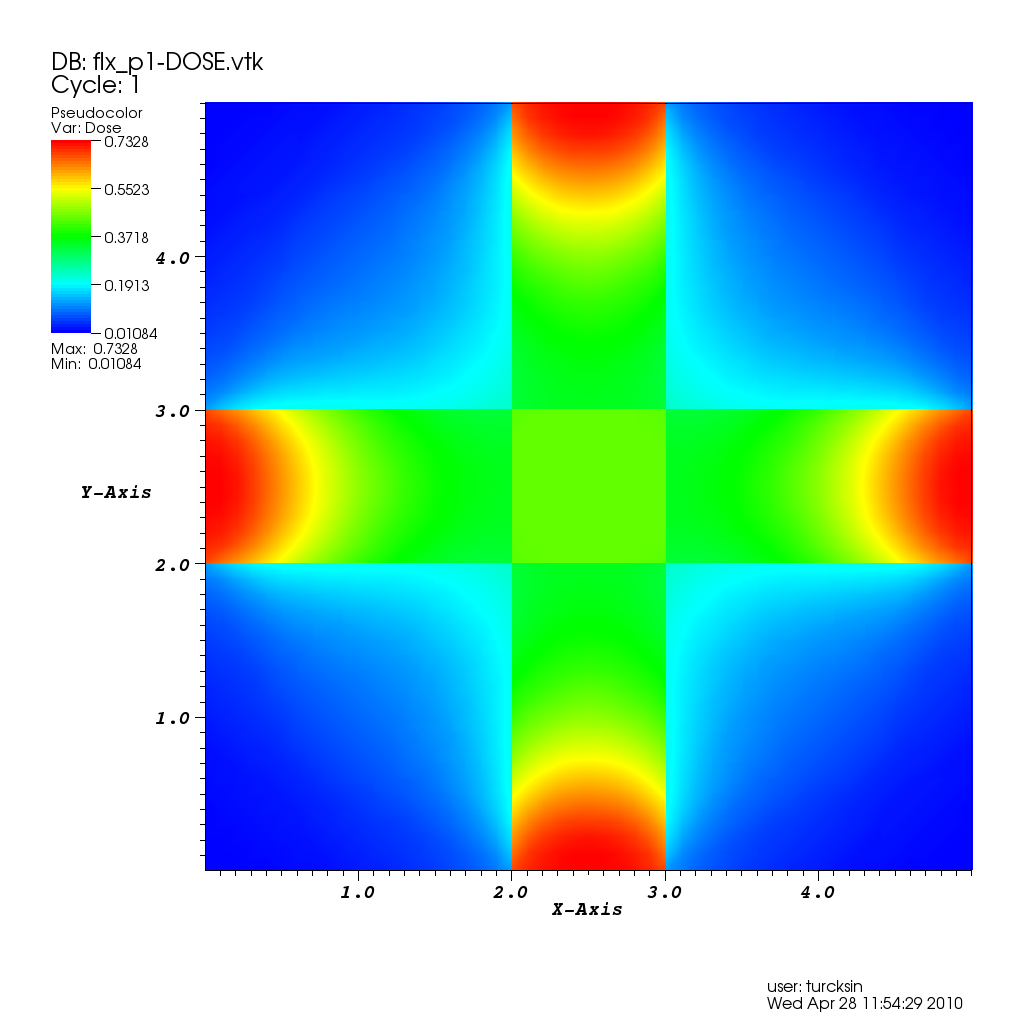
\includegraphics[width=0.5\linewidth]{L_M_D_V}
\end{figure}
We have only 4 beams which are turned on, with the following intensities : 2.1875. We should notice that now we have the same intensity for the 4 beams. For the first objective function, the 4 beams have different values. We need only 73 seconds to solve the problem. So we see that we save a lot time by using our own method instead of using the function of the Python library (Scipy). The value of the objective function is 0.31 and the dose in the middle cell is 0.44. Here, we should notice that if we add to the ``unconstrained'' Hessian the identity matrix multiply by $10^{-8}$, there is no problem. However, if we add another number, we will impose more constrained than we have parameters (intensity of the beams) and the matrix will become singular. It is probably because some of the constraints are degenerated. Effectively, sometimes we add some constraints but the step to reach that constraint is almost 0 ($10^{-14}$ times smaller than the others). Thus, we add a constraint and we don't move. So the degeneration of the constraints might be a possible explanation. The other is that there is a bug but the result seems good. When we choose to add $10^{-8}$ to the matrix, the method has the behavior that we could expect :
\begin{enumerate}
\item We start from an intensity of 0 and then we increase the intensity of all the beams like in the unconstrained case
\item We cannot increase the intensity because of the constraints on the maximum dose and we add the constraints of maximum dose
\item We increase the value of the 4 middle beams and we decrease the intensity of the others. We release some of the constraints of maximum dose and we add the constraints of the positive intensity.
\end{enumerate}
For the others values, it does not work so nicely. We fixed the problem by adding an identity matrix multiplied by $10^{-8}$ on the zero submatrix of the left-hand side. With that modification we can choose the value that we need to add on the diagonal of the Hessian. We always find the same results than before which is the one we expected. 
\subsubsection{Scaling method}
First we should notice that if we do not add elements on the zero submatrix, the matrix will become singular. We show here the result when we multiply the diagonal of the matrix by $1+10^{-6}$ \footnote{The result for $1+10^{-8}$ are similar} :
\begin{figure}[H]
\centering
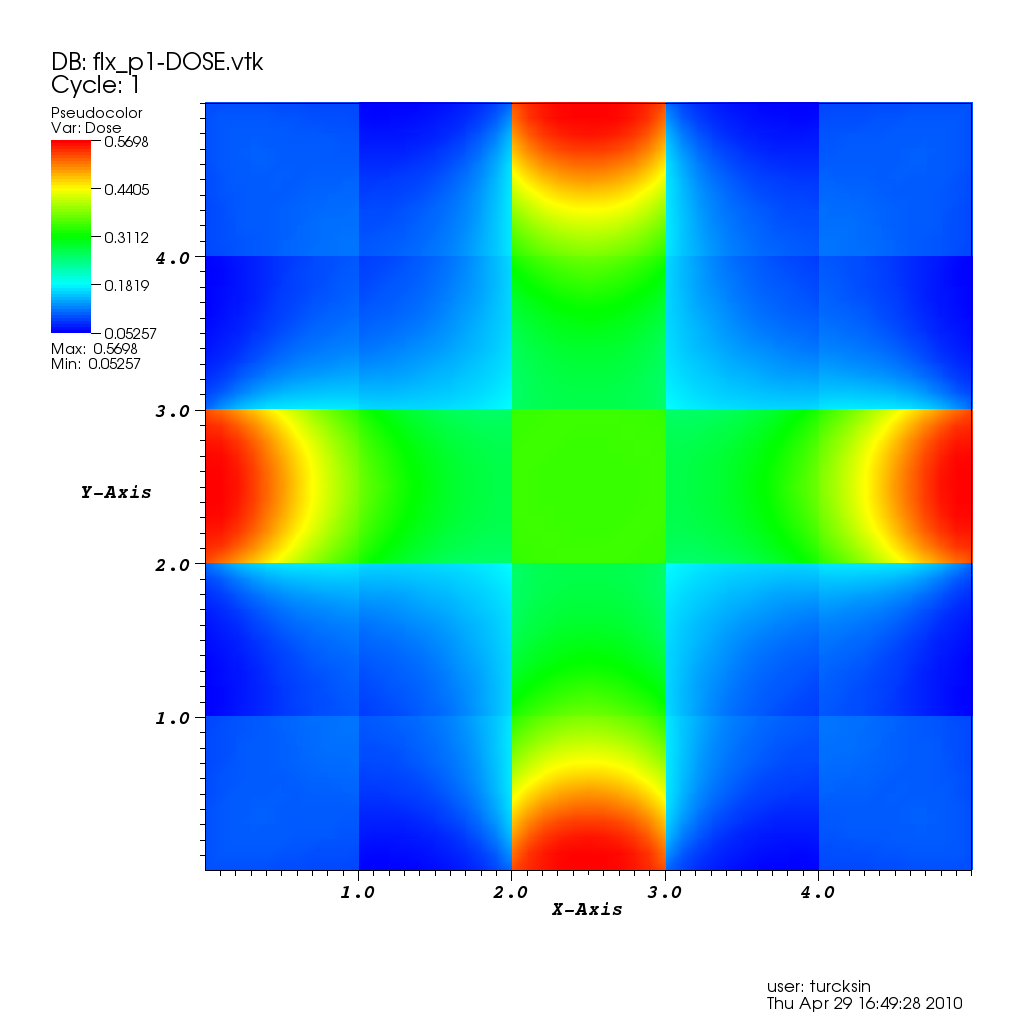
\includegraphics[width=0.5\linewidth]{1e-6}
\end{figure}
We see that we have a result which is close of what we had before. On the corner, the intensity of the beams is 0.144. On the middle the intensity of the beams is 1.663. The others are 0. The value of the objective function is : 0.434. The dose in the target is 0.3413 and it take 93s to have the results. The reason why it takes more time than before is the following : in this problem, it happens that the following step of the Newton method is very small. Thus, we iterate until we reach the maximum number of iterations, then we recompute the new constraints and we restart the Newton's method. In the previous method, we never reach the maximum number of iterations.\\

If we multiply the diagonal by $1+10^{-10}$, we find :
\begin{figure}[H]
\centering
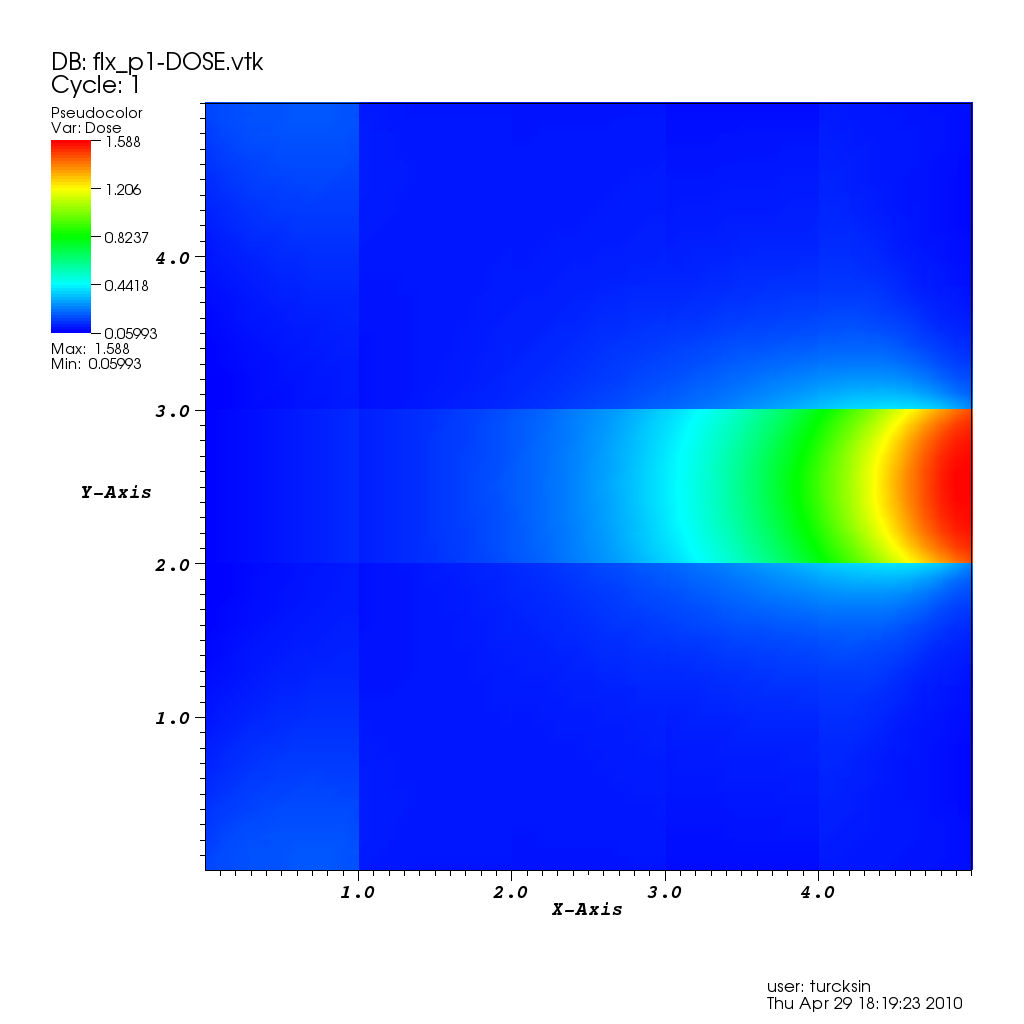
\includegraphics[width=0.5\linewidth]{1e-10}
\end{figure}
We have a result which is very strange : the right beam has an intensity of 5.73, the left beam has en intensity of 0.093 and the top and the bottom beams of the left have an intensity of 0.356. The value of the objective function is 0.494 and the dose in the target is 0.284. It takes 93s to have the results.

\subsection{Cross target}
Now we show one last example, the target as the shape of a cross :
\begin{figure}[H]
\centering
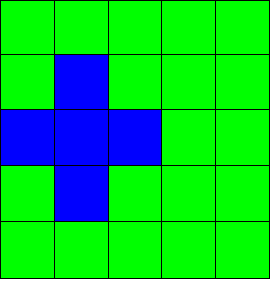
\includegraphics[width=0.2\linewidth]{schema1}
\end{figure}
We allow 30\% of the healthy cells (6 cells) to receive a dose higher than 0.1. First we will look at the unconstrained problem :
\begin{figure}[H]
\centering
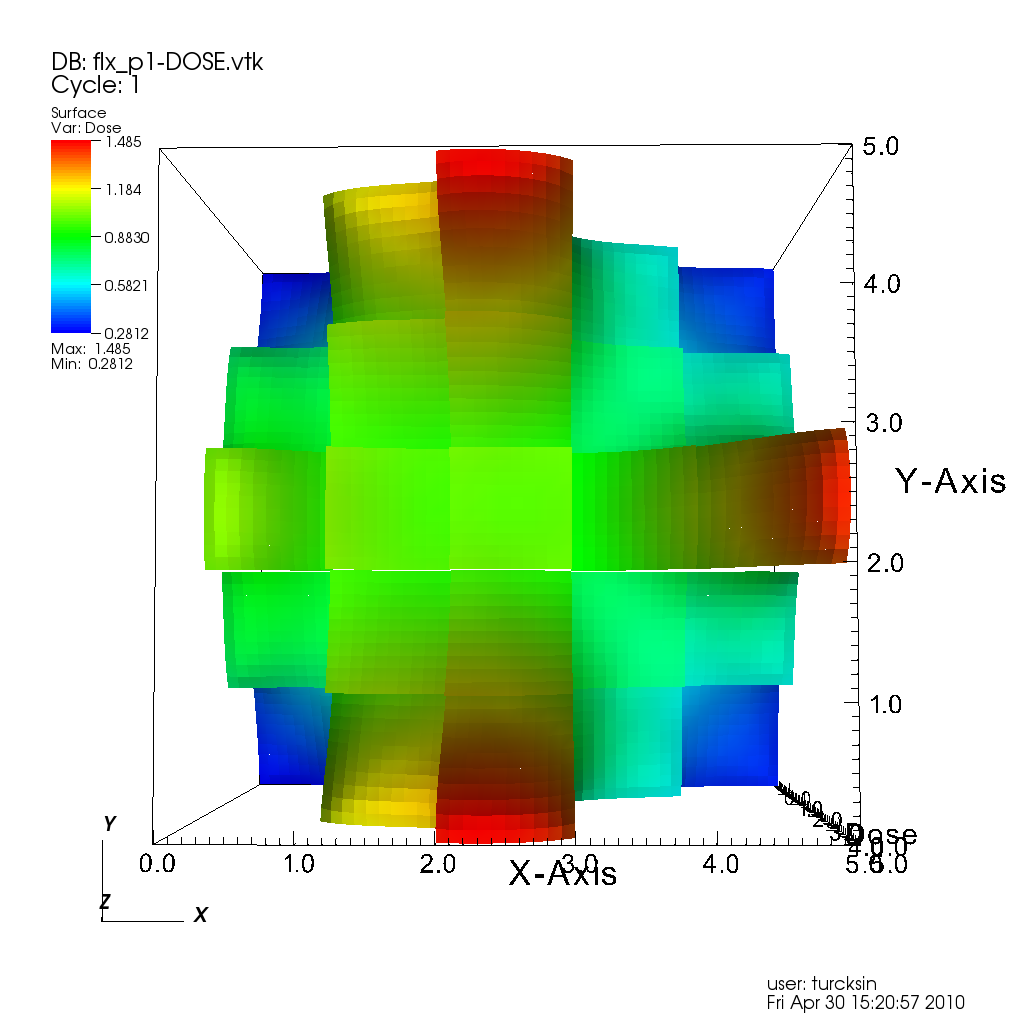
\includegraphics[width=0.5\linewidth]{lastunc}
\end{figure}
The result seems weird at first sight but it is easy to explain. The beam in the middle left is not very high because it just needs to give a dose of 1 to the cell of the target. The beam on the top and the one on the bottom which are aligned on the target, give the dose on that column of cells. The 3 others beams give the dose in the middle cells. Now we can understand the result of the constrained problem :
\begin{figure}[H]
\centering
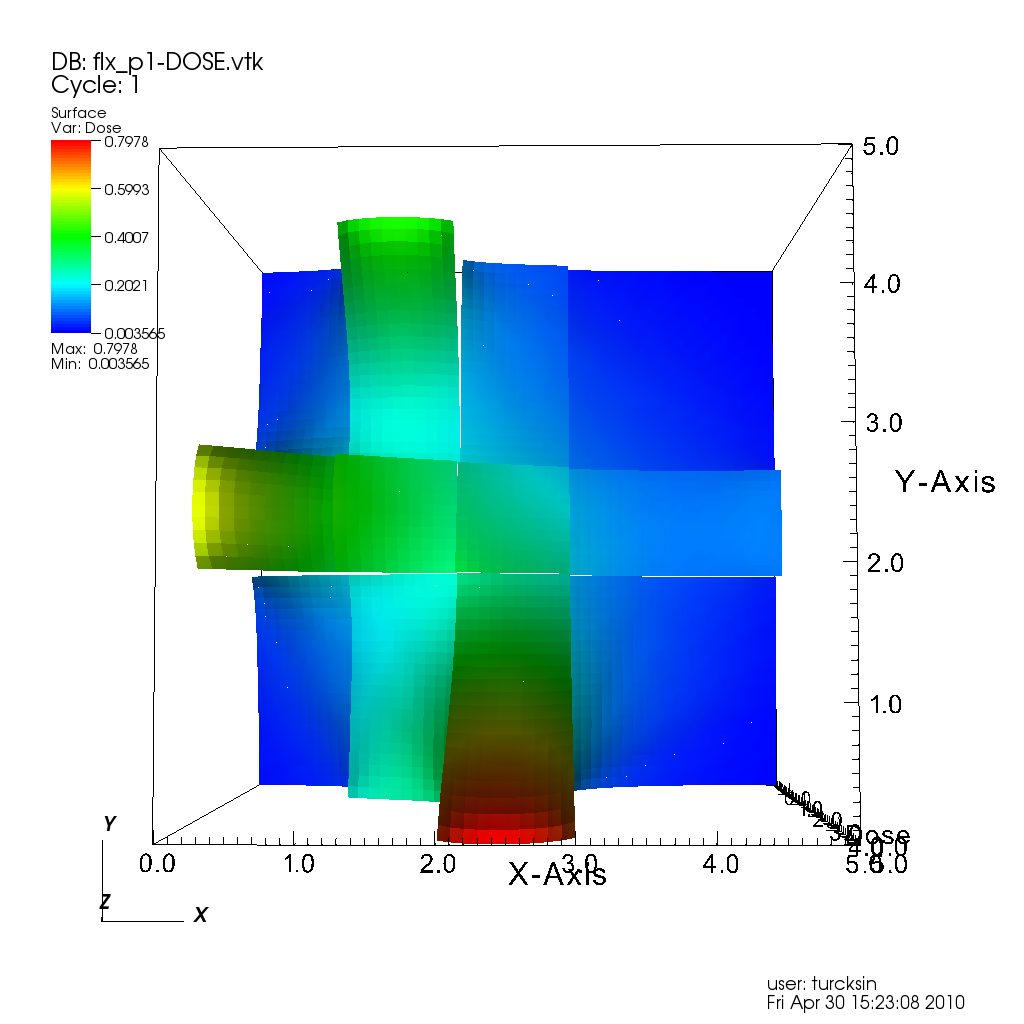
\includegraphics[width=0.5\linewidth]{lastcons}
\end{figure}
The beam on the left gives the dose for the cells in the middle row. The 2 beams on the top and the middle give the dose on that row of the target. The beams on the middle, bottom and right, give the dose of the cell in the middle of the square. The dose in the target is 0.23, 0.48, 0.34, 0.25 and 0.22. The dose is thus much lower that what we wanted. Below we show the cells which receives an higher dose than the maximum :
\begin{figure}[H]
\centering
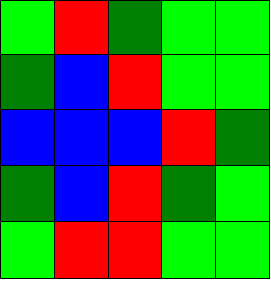
\includegraphics[width=0.2\linewidth]{schema2}
\end{figure}
The blue is target, the light green cells are the healthy cells which receive less than the maximum dose, the dark green cells are the healthy cells which receive the maximum dose that we allow and in red we have the cells which receive a dose higher than what allowed. Now we can understand why the beam on the bottom left is weaker than the one on the top. If we increase a little bit the intensity of the beam, the cell on the left will receive a dose bigger than the limit.\\

This solution is probably not the global minimum. The value of the objective function could be smaller if we were using 3 beams on the left and the 2 beams on the top and the bottom of the target. However, we should notice that the method escaped from one local minima before to get stuck in the other.

\section{Conclusions}
The first objective function was easy to implement since we could use a library in Python which solves the problem. However, using this objective function is annoying since we don't know which factors $\theta$ we need to use. The time needed to solve the problem can easily be decreased. What we must do is very similar of what we do to solve the unconstrained problem of the second objective function. The objective function is different but we can form the Hessian once and then solve the problem. We can expect to solve the problem in about the same time we needed for the Levenberg-Marquardt method (we spend most of our time to compute the gradient of the flux).\\

For the second objective function, it is important to see that the difficulty arises because the function is positive semi-positive (we need to change the Hessian) and the constraints are not convex (there are some local minima). Most of the time people use stochastic methods to find the global minima (however there is some deterministic methods \cite{livre}). Here we tried to find a good approximation of the global minimum using a deterministic method. We found the global minimum only when the solution is close to the solution of the unconstrained problem. Moreover we saw that we need to be very careful when we change the Hessian. We cannot perturb the Hessian in an arbitrary way and expect to have the right result. 

\newpage
\bibliographystyle{unsrt}
\bibliography{biblio}

\end{document}
